\documentclass{article}\usepackage[]{graphicx}\usepackage[]{color}
%% maxwidth is the original width if it is less than linewidth
%% otherwise use linewidth (to make sure the graphics do not exceed the margin)
\makeatletter
\def\maxwidth{ %
  \ifdim\Gin@nat@width>\linewidth
    \linewidth
  \else
    \Gin@nat@width
  \fi
}
\makeatother

\definecolor{fgcolor}{rgb}{0.345, 0.345, 0.345}
\newcommand{\hlnum}[1]{\textcolor[rgb]{0.686,0.059,0.569}{#1}}%
\newcommand{\hlstr}[1]{\textcolor[rgb]{0.192,0.494,0.8}{#1}}%
\newcommand{\hlcom}[1]{\textcolor[rgb]{0.678,0.584,0.686}{\textit{#1}}}%
\newcommand{\hlopt}[1]{\textcolor[rgb]{0,0,0}{#1}}%
\newcommand{\hlstd}[1]{\textcolor[rgb]{0.345,0.345,0.345}{#1}}%
\newcommand{\hlkwa}[1]{\textcolor[rgb]{0.161,0.373,0.58}{\textbf{#1}}}%
\newcommand{\hlkwb}[1]{\textcolor[rgb]{0.69,0.353,0.396}{#1}}%
\newcommand{\hlkwc}[1]{\textcolor[rgb]{0.333,0.667,0.333}{#1}}%
\newcommand{\hlkwd}[1]{\textcolor[rgb]{0.737,0.353,0.396}{\textbf{#1}}}%
\let\hlipl\hlkwb

\usepackage{framed}
\makeatletter
\newenvironment{kframe}{%
 \def\at@end@of@kframe{}%
 \ifinner\ifhmode%
  \def\at@end@of@kframe{\end{minipage}}%
  \begin{minipage}{\columnwidth}%
 \fi\fi%
 \def\FrameCommand##1{\hskip\@totalleftmargin \hskip-\fboxsep
 \colorbox{shadecolor}{##1}\hskip-\fboxsep
     % There is no \\@totalrightmargin, so:
     \hskip-\linewidth \hskip-\@totalleftmargin \hskip\columnwidth}%
 \MakeFramed {\advance\hsize-\width
   \@totalleftmargin\z@ \linewidth\hsize
   \@setminipage}}%
 {\par\unskip\endMakeFramed%
 \at@end@of@kframe}
\makeatother

\definecolor{shadecolor}{rgb}{.97, .97, .97}
\definecolor{messagecolor}{rgb}{0, 0, 0}
\definecolor{warningcolor}{rgb}{1, 0, 1}
\definecolor{errorcolor}{rgb}{1, 0, 0}
\newenvironment{knitrout}{}{} % an empty environment to be redefined in TeX

\usepackage{alltt}

\usepackage{fancyhdr} % Required for custom headers
\usepackage{lastpage} % Required to determine the last page for the footer
\usepackage{extramarks} % Required for headers and footers
\usepackage{graphicx} % Required to insert images
\usepackage{hyperref}
\usepackage{amsmath} %for binomial pdf
\usepackage{parskip} % so that there's space bw paragraphs
\usepackage{float}
\usepackage{amsfonts}

% Margins
\topmargin=-0.45in
\evensidemargin=0in
\oddsidemargin=0in
\textwidth=6.5in
\textheight=9.0in
\headsep=0.25in 

\linespread{1.1} % Line spacing

% Set up the header and footer
\pagestyle{fancy}
\lhead{STAT 534: Spatial} % Top left header
\chead{HW 3} % Top center header
\rhead{Andrea Mack} % Top right header
\lfoot{01/30/2017} % Bottom left footer
\cfoot{} % Bottom center footer
\rfoot{Page\ \thepage\ of\ \pageref{LastPage}} % Bottom right footer
\renewcommand\headrulewidth{0.4pt} % Size of the header rule
\renewcommand\footrulewidth{0.4pt} % Size of the footer rule

\setlength\parindent{0pt} % Removes all indentation from paragraphs
\setlength\parskip{0.5cm}
\restylefloat{table}

%----------------------------------------------------------------------------------------
%	DOCUMENT STRUCTURE COMMANDS
%	Skip this unless you know what you're doing
%----------------------------------------------------------------------------------------

% Header and footer for when a page split occurs within a problem environment
\newcommand{\enterProblemHeader}[1]{
\nobreak\extramarks{#1}{#1 continued on next page\ldots}\nobreak
\nobreak\extramarks{#1 (continued)}{#1 continued on next page\ldots}\nobreak
}

% Header and footer for when a page split occurs between problem environments
\newcommand{\exitProblemHeader}[1]{
\nobreak\extramarks{#1 (continued)}{#1 continued on next page\ldots}\nobreak
\nobreak\extramarks{#1}{}\nobreak
}


%----------------------------------------------------------------------------------------%
\IfFileExists{upquote.sty}{\usepackage{upquote}}{}
\begin{document}



\begin{enumerate}
\item %1
{\it On the last homework there was some confusion about two problems. I took o↵ some points for one of those but am now giving you a chance to get them back.}

\begin{enumerate}
\item %1a
{\it It was pointed out in class that, conditional on n events, event locations are uniformly distributed for a homogeneous Poisson process. Show this result for a 1   d process. Hint: Consider a one-dimensional process on a transect of length L, (0,L]. Given that one event has occurred on the interval (0,L] what is the probability that it occurred in the subinterval (0, s] for s \textless L? Show that this is the cdf of a Unif (0,L) distribution.}

\vspace{3in}

\item %1b
{\it Suppose we have a realization of a spatial point process consisting of N event locations {s1, s2, · · · , sN }. Let Hi denote the distance between the ith event and the nearest neigh- boring event. The cumulative distribution function of H (the nearest event-event dis- tance) is the G function. (This problem will be continued on the next homework assignment). Derive the G function if the point process is CSR; i.e. what is G(h) = P (H $\leq$ h).}

\vspace{4in}

\end{enumerate}

\item %2
{\it We looked at one simple method of using nearest neighbor distances to assess a null hypothesis of CSR. The method was based on using Monte Carlo tests to evaluate the deviation of the mean distance from that expected under CSR. We will look at another possible approach in this problem, one that theoretically would allow us to use a test based on normal theory. A question on Homework 2 asked you to find the probability density function of H, the distance between an event and the nearest neighboring event.}

{\it We will be working with a homogeneous Poisson process with intensity $\lambda$  = 30.}
\begin{enumerate}
\item %2a
{\it What are the mean and variance of $\bar{H}$ = $\frac{1}{30}\Sigma H_{i}$ when $\lambda$ = 30, ie.e both the sample size and the intensity equal 30.}


$\beta = 2$; $\theta = (\lambda\pi)^{\frac{-1}{2}}$; $\lambda = n = 30$

$E[\bar{H}]$ = $\frac{1}{n}E[\Sigma{\bar{H}}]$ = $E[H]$ = $\theta * \Gamma[1 + \frac{1}{\beta}]$

$\rightarrow E[\bar{H}]$ = $(30\pi)^{-\frac{1}{2}}\Gamma(\frac{3}{2})$ = $(30\pi)^{-\frac{1}{2}}\frac{1}{2}\Gamma(\frac{1}{2})$ = $(30^{2}\pi)^{-1}\frac{1}{2}(\pi)^{\frac{1}{2}}$ = $\frac{1}{2*(30)^{2}}$ $\approx 0.0913$

$Var[\bar{H}] = \frac{1}{n}Var[H]$ = $\frac{\theta^{2}[\Gamma(1+\frac{2}{\beta}) - (\Gamma(1+\frac{1}{\beta}))^{2}]}{n}$ = $30*[\Gamma(2) - (\frac{1}{2}\Gamma(\frac{1}{2})^{2}]$ = $\frac{1}{30^{2}\pi}[1-\frac{1}{4}\pi]$ $\approx$ $\ensuremath{10^{-4}}$

\item %2b
{\it What is the approximate sampling distribution of $Z = \frac{\bar{H} - E[\bar{H}]}{(Var[\bar{H}])^{\frac{1}{2}}}$ under CSR and how do you know this?} 

Note that $\beta = 2 \geq 1 \rightarrow$ the mgf exists. By the CLT, $\frac{\bar{H} - E[\bar{H}]}{(Var[\bar{H}])^{\frac{1}{2}}} \rightarrow N(0,1)$.

\item %2c
{\it Simulate 1000 realizations of complete spatial randomness in the unit square with 30 events in each realization. For each realization}

\begin{enumerate}
\item %2ci
{\it Calculate the distance between each event and its nearest-neighboring event (Hi for the ith event in the realization)}

\begin{knitrout}\footnotesize
\definecolor{shadecolor}{rgb}{0.969, 0.969, 0.969}\color{fgcolor}\begin{kframe}
\begin{alltt}
\hlstd{csr_sim30} \hlkwb{<-} \hlkwd{array}\hlstd{(}\hlnum{0}\hlstd{,}\hlkwd{c}\hlstd{(}\hlnum{30}\hlstd{,}\hlnum{2}\hlstd{,}\hlnum{1000}\hlstd{))}
\hlstd{csr_nndist} \hlkwb{<-} \hlkwd{data.frame}\hlstd{(}\hlkwd{matrix}\hlstd{(}\hlnum{0}\hlstd{,}\hlkwc{nrow} \hlstd{=} \hlnum{30}\hlstd{,} \hlkwc{ncol}\hlstd{=}\hlnum{1000}\hlstd{))}
\hlkwd{set.seed}\hlstd{(}\hlnum{123}\hlstd{)}
\hlkwa{for}\hlstd{(i} \hlkwa{in} \hlnum{1}\hlopt{:}\hlnum{1000}\hlstd{)\{}
  \hlstd{re} \hlkwb{<-} \hlkwd{runifpoint}\hlstd{(}\hlnum{30}\hlstd{,} \hlkwc{win}\hlstd{=}\hlkwd{owin}\hlstd{(}\hlkwd{c}\hlstd{(}\hlnum{0}\hlstd{,}\hlnum{1}\hlstd{),}\hlkwd{c}\hlstd{(}\hlnum{0}\hlstd{,}\hlnum{1}\hlstd{)))}
  \hlstd{csr_sim30[,,i]} \hlkwb{<-} \hlkwd{c}\hlstd{(re}\hlopt{$}\hlstd{x,re}\hlopt{$}\hlstd{y)}
\hlstd{\}}
\end{alltt}
\end{kframe}
\end{knitrout}

\begin{knitrout}\footnotesize
\definecolor{shadecolor}{rgb}{0.969, 0.969, 0.969}\color{fgcolor}\begin{kframe}
\begin{alltt}
\hlstd{csr_nndist} \hlkwb{<-} \hlkwd{apply}\hlstd{(csr_sim30,}\hlnum{3}\hlstd{,nndist)}
\end{alltt}
\end{kframe}
\end{knitrout}

\item %2cii
{\it Calculate and store the mean distance.}

\begin{knitrout}\footnotesize
\definecolor{shadecolor}{rgb}{0.969, 0.969, 0.969}\color{fgcolor}\begin{kframe}
\begin{alltt}
\hlstd{nndist_mean} \hlkwb{<-} \hlkwd{c}\hlstd{(}\hlkwd{colMeans}\hlstd{(csr_nndist))}
\end{alltt}
\end{kframe}
\end{knitrout}

\item %2ciii
{\it Calculate and store the values of Z using the mean and variance from part (a) above.}

\begin{knitrout}\footnotesize
\definecolor{shadecolor}{rgb}{0.969, 0.969, 0.969}\color{fgcolor}\begin{kframe}
\begin{alltt}
\hlstd{Z} \hlkwb{<-} \hlstd{(nndist_mean} \hlopt{-} \hlstd{e_hbar)}\hlopt{/}\hlstd{sd_hbar}
\end{alltt}
\end{kframe}
\end{knitrout}
\end{enumerate}
\newpage

\item %2d
{\it Compute the mean and standard deviation of the 1000 simulated H values and compare them to what would be expected under CSR. Are they higher or lower than expected? What could explain this result?}

The theoretical values are slightly smaller. That may happen because assuming the nearest neighbor distances are within a circle will give slightly smaller nearest neighbor distances on average than looking at points in a square because the circle fits inside the square, leaving the corners of the square unattainable under the theoretical calculation. The correction adjusts to use the area and perimeter of a unitized square, which is what was used to simulate points.

\begin{kframe}
\begin{alltt}
\hlstd{emp_mean} \hlkwb{<-} \hlkwd{mean}\hlstd{(nndist_mean)}
\hlstd{emp_sd} \hlkwb{<-} \hlkwd{sqrt}\hlstd{(}\hlkwd{var}\hlstd{(nndist_mean))}

\hlstd{all_hbar} \hlkwb{<-} \hlkwd{data.frame}\hlstd{(}\hlkwd{matrix}\hlstd{(}\hlkwd{c}\hlstd{(emp_mean, e_hbar, emp_sd, sd_hbar),} \hlkwc{nrow} \hlstd{=} \hlnum{2}\hlstd{,} \hlkwc{ncol} \hlstd{=} \hlnum{2}\hlstd{,} \hlkwc{byrow} \hlstd{=} \hlnum{TRUE}\hlstd{))}
\hlkwd{rownames}\hlstd{(all_hbar)} \hlkwb{<-} \hlkwd{c}\hlstd{(}\hlstr{"Mean(Hbar)"}\hlstd{,} \hlstr{"SD(Hbar)"}\hlstd{)}
\hlkwd{colnames}\hlstd{(all_hbar)} \hlkwb{<-} \hlkwd{c}\hlstd{(}\hlstr{"Simulated"}\hlstd{,} \hlstr{"Theoretical"}\hlstd{)}

\hlkwd{print}\hlstd{(}\hlkwd{xtable}\hlstd{(all_hbar,} \hlkwc{align} \hlstd{=} \hlstr{"||l|l|l||"}\hlstd{,}\hlkwc{digits}\hlstd{=}\hlkwd{c}\hlstd{(}\hlnum{4}\hlstd{,}\hlnum{4}\hlstd{,}\hlnum{4}\hlstd{)))}
\end{alltt}
\end{kframe}% latex table generated in R 3.3.2 by xtable 1.8-2 package
% Fri Feb  3 11:41:25 2017
\begin{table}[ht]
\centering
\begin{tabular}{||l|l|l||}
  \hline
 & Simulated & Theoretical \\ 
  \hline
Mean(Hbar) & 0.0994 & 0.0913 \\ 
  SD(Hbar) & 0.0104 & 0.0100 \\ 
   \hline
\end{tabular}
\end{table}


\item %2e
{\it Produce a qqplot of the z scores. Comment.}

The theoretical quantiles and the observed quantiles fall on a straight line with slight deviations at the tails. This suggests normality is reasonable with possibly some edge effects.



\begin{knitrout}\footnotesize
\definecolor{shadecolor}{rgb}{0.969, 0.969, 0.969}\color{fgcolor}\begin{kframe}
\begin{alltt}
\hlkwd{qqnorm}\hlstd{(Z,} \hlkwc{xlab} \hlstd{=} \hlstr{"Theoretical"}\hlstd{,} \hlkwc{ylab} \hlstd{=} \hlstr{"Observed"}\hlstd{,} \hlkwc{main} \hlstd{=} \hlstr{"Normal Q-Q for Z"}\hlstd{)}
\end{alltt}
\end{kframe}

{\centering 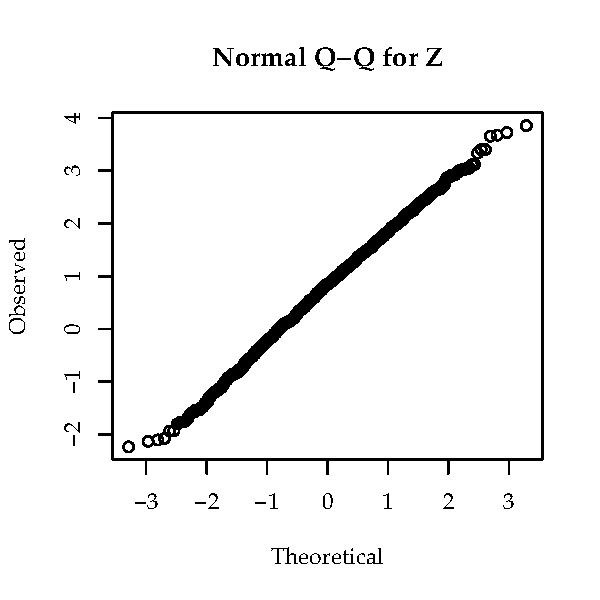
\includegraphics[width=\maxwidth]{figure/prob2e-1} 

}


\begin{kframe}\begin{alltt}
\hlcom{#abline(0,1,col=2)}
\end{alltt}
\end{kframe}
\end{knitrout}
\newpage

\item %2f
{\it Use the following formulas for the expected value and variance of $\bar{H}$:}

{\it where A is the area and P is the perimeter of the spatial domain (the unit square). Compare the mean and standard deviation from these formulas to those you computed from the simulations above. Does this modification seem to help?}

The modification seems to correct for discrepancies.
\begin{kframe}
\begin{alltt}
\hlstd{A} \hlkwb{<-} \hlnum{1}
\hlstd{P} \hlkwb{<-} \hlnum{4}
\hlstd{n} \hlkwb{<-} \hlkwd{nrow}\hlstd{(csr_sim30)}

\hlstd{e_hbar1} \hlkwb{<-} \hlnum{0.5}\hlopt{*}\hlkwd{sqrt}\hlstd{(A}\hlopt{/}\hlstd{n)} \hlopt{+} \hlnum{0.051}\hlopt{*}\hlstd{(P}\hlopt{/}\hlstd{n)} \hlopt{+} \hlnum{0.041}\hlopt{*}\hlstd{P}\hlopt{/}\hlstd{n}\hlopt{^}\hlstd{(}\hlnum{3}\hlopt{/}\hlnum{2}\hlstd{)}
\hlstd{var_hbar1} \hlkwb{<-} \hlnum{0.0703}\hlopt{*}\hlstd{A}\hlopt{/}\hlstd{n}\hlopt{^}\hlnum{2} \hlopt{+} \hlnum{0.037}\hlopt{*}\hlstd{P}\hlopt{*}\hlkwd{sqrt}\hlstd{(A}\hlopt{/}\hlstd{n}\hlopt{^}\hlnum{5}\hlstd{)}

\hlstd{all_plus} \hlkwb{<-} \hlkwd{data.frame}\hlstd{(}\hlkwd{cbind}\hlstd{(all_hbar,}\hlkwd{c}\hlstd{(e_hbar1,}\hlkwd{sqrt}\hlstd{(var_hbar1))))}
\hlkwd{rownames}\hlstd{(all_plus)} \hlkwb{<-} \hlkwd{rownames}\hlstd{(all_hbar)}
\hlkwd{colnames}\hlstd{(all_plus)} \hlkwb{<-} \hlkwd{c}\hlstd{(}\hlstr{"Simulated"}\hlstd{,} \hlstr{"Theoretical"}\hlstd{,} \hlstr{"Corrected"}\hlstd{)}

\hlkwd{print}\hlstd{(}\hlkwd{xtable}\hlstd{(all_plus,} \hlkwc{align} \hlstd{=} \hlstr{"||l|l|l|l||"}\hlstd{,} \hlkwc{digits} \hlstd{=} \hlkwd{c}\hlstd{(}\hlnum{5}\hlstd{,}\hlnum{5}\hlstd{,}\hlnum{5}\hlstd{,}\hlnum{5}\hlstd{)))}
\end{alltt}
\end{kframe}% latex table generated in R 3.3.2 by xtable 1.8-2 package
% Fri Feb  3 11:41:25 2017
\begin{table}[ht]
\centering
\begin{tabular}{||l|l|l|l||}
  \hline
 & Simulated & Theoretical & Corrected \\ 
  \hline
Mean(Hbar) & 0.09939 & 0.09130 & 0.09909 \\ 
  SD(Hbar) & 0.01040 & 0.01000 & 0.01040 \\ 
   \hline
\end{tabular}
\end{table}


\item %2g
{\it The above procedure is called the Clark-Evans test. Use it to test the null hypothesis of CSR for the cells and redwood data sets. Interpret the results of each test. Also, compute approximate large sample 95\% confidence intervals for the mean distance and interpret.}

\begin{knitrout}\footnotesize
\definecolor{shadecolor}{rgb}{0.969, 0.969, 0.969}\color{fgcolor}\begin{kframe}
\begin{alltt}
\hlkwd{data}\hlstd{(}\hlstr{"cells"}\hlstd{)}
\hlstd{csr_cells} \hlkwb{<-} \hlkwd{array}\hlstd{(}\hlnum{0}\hlstd{,}\hlkwd{c}\hlstd{(cells}\hlopt{$}\hlstd{n,} \hlnum{2}\hlstd{,} \hlnum{1000}\hlstd{))}
\hlstd{nndist_cells} \hlkwb{<-} \hlkwd{data.frame}\hlstd{(}\hlkwd{matrix}\hlstd{(}\hlnum{0}\hlstd{,}\hlkwc{nrow} \hlstd{= cells}\hlopt{$}\hlstd{n,} \hlkwc{ncol}\hlstd{=}\hlnum{1000}\hlstd{))}

\hlkwd{set.seed}\hlstd{(}\hlnum{123}\hlstd{)}
\hlkwa{for}\hlstd{(i} \hlkwa{in} \hlnum{1}\hlopt{:}\hlnum{1000}\hlstd{)\{}
  \hlstd{re} \hlkwb{<-} \hlkwd{runifpoint}\hlstd{(}\hlnum{42}\hlstd{,} \hlkwc{win}\hlstd{=}\hlkwd{owin}\hlstd{(}\hlkwd{c}\hlstd{(}\hlnum{0}\hlstd{,}\hlnum{1}\hlstd{),}\hlkwd{c}\hlstd{(}\hlnum{0}\hlstd{,}\hlnum{1}\hlstd{)))}
  \hlstd{csr_cells[,,i]} \hlkwb{<-} \hlkwd{c}\hlstd{(re}\hlopt{$}\hlstd{x,re}\hlopt{$}\hlstd{y)}
\hlstd{\}}


\hlstd{nndist_cells} \hlkwb{<-} \hlkwd{apply}\hlstd{(csr_cells,}\hlnum{3}\hlstd{,nndist)}
\hlstd{mean_cells} \hlkwb{<-} \hlstd{(}\hlkwd{colMeans}\hlstd{(nndist_cells))}

\hlcom{# the cell data were rescaled to the unit square}
\hlstd{A} \hlkwb{<-} \hlnum{1}
\hlstd{P} \hlkwb{<-} \hlnum{4}
\hlstd{n.cells} \hlkwb{<-} \hlkwd{nrow}\hlstd{(csr_cells)}

\hlstd{e_hbar.cells} \hlkwb{<-} \hlnum{0.5}\hlopt{*}\hlkwd{sqrt}\hlstd{(A}\hlopt{/}\hlstd{n.cells)} \hlopt{+} \hlnum{0.051}\hlopt{*}\hlstd{(P}\hlopt{/}\hlstd{n.cells)} \hlopt{+} \hlnum{0.041}\hlopt{*}\hlstd{P}\hlopt{/}\hlstd{n.cells}\hlopt{^}\hlstd{(}\hlnum{3}\hlopt{/}\hlnum{2}\hlstd{)}
\hlstd{var_hbar.cells} \hlkwb{<-} \hlnum{0.0703}\hlopt{*}\hlstd{A}\hlopt{/}\hlstd{n.cells}\hlopt{^}\hlnum{2} \hlopt{+} \hlnum{0.037}\hlopt{*}\hlstd{P}\hlopt{*}\hlkwd{sqrt}\hlstd{(A}\hlopt{/}\hlstd{n.cells}\hlopt{^}\hlnum{5}\hlstd{)}
\hlstd{sd_hbar.cells} \hlkwb{<-} \hlkwd{sqrt}\hlstd{(var_hbar.cells)}
\hlstd{Z_cells} \hlkwb{<-} \hlstd{(mean_cells} \hlopt{-} \hlstd{e_hbar.cells)}\hlopt{/}\hlstd{sd_hbar.cells}

\hlkwd{qqnorm}\hlstd{(Z_cells,} \hlkwc{main} \hlstd{=} \hlstr{"Q-Q Norm Clark-Evans Cells"}\hlstd{)}
\hlkwd{abline}\hlstd{(}\hlkwc{a}\hlstd{=}\hlnum{0}\hlstd{,}\hlkwc{b}\hlstd{=}\hlnum{1}\hlstd{,}\hlkwc{col}\hlstd{=}\hlnum{2}\hlstd{)}
\end{alltt}
\end{kframe}

{\centering 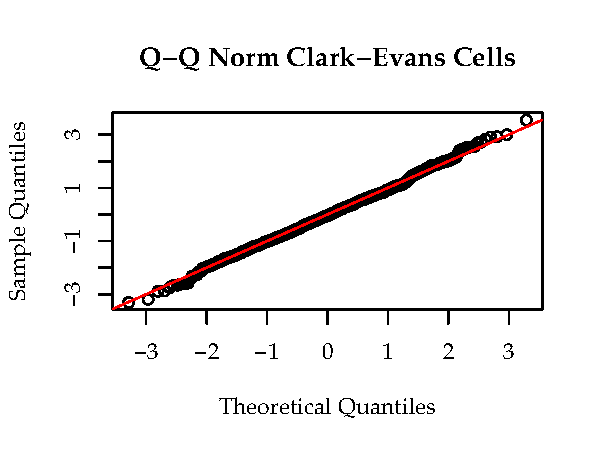
\includegraphics[width=\maxwidth]{figure/prob2g_cells-1} 

}



\end{knitrout}

\begin{kframe}
\begin{alltt}
\hlstd{obs_cells} \hlkwb{<-} \hlkwd{nndist}\hlstd{(cells)}
\hlstd{obs_mean.cells} \hlkwb{<-} \hlkwd{mean}\hlstd{(obs_cells)}
\hlstd{obs_sd.cells} \hlkwb{<-} \hlkwd{sqrt}\hlstd{(}\hlkwd{var}\hlstd{(obs_cells))}

\hlstd{all_cells} \hlkwb{<-} \hlkwd{data.frame}\hlstd{(}\hlkwd{cbind}\hlstd{(}\hlkwd{c}\hlstd{(obs_mean.cells,obs_sd.cells),}\hlkwd{c}\hlstd{(}\hlkwd{mean}\hlstd{(mean_cells),} \hlkwd{sqrt}\hlstd{(}\hlkwd{var}\hlstd{(mean_cells))),} \hlkwd{c}\hlstd{(e_hbar.cells,}\hlkwd{sqrt}\hlstd{(var_hbar.cells))))}
\hlkwd{rownames}\hlstd{(all_cells)} \hlkwb{<-} \hlkwd{rownames}\hlstd{(all_hbar)}
\hlkwd{colnames}\hlstd{(all_cells)} \hlkwb{<-} \hlkwd{c}\hlstd{(}\hlstr{"Observed"}\hlstd{,} \hlstr{"Simulated"}\hlstd{,} \hlstr{"Corrected"}\hlstd{)}

\hlkwd{print}\hlstd{(}\hlkwd{xtable}\hlstd{(all_cells,} \hlkwc{align} \hlstd{=} \hlstr{"||l|l|l|l||"}\hlstd{,} \hlkwc{digits} \hlstd{=} \hlkwd{c}\hlstd{(}\hlnum{5}\hlstd{,}\hlnum{5}\hlstd{,}\hlnum{5}\hlstd{,}\hlnum{5}\hlstd{),} \hlkwc{caption} \hlstd{=} \hlstr{"Cells"}\hlstd{))}
\end{alltt}
\end{kframe}% latex table generated in R 3.3.2 by xtable 1.8-2 package
% Fri Feb  3 11:41:26 2017
\begin{table}[ht]
\centering
\begin{tabular}{||l|l|l|l||}
  \hline
 & Observed & Simulated & Corrected \\ 
  \hline
Mean(Hbar) & 0.12897 & 0.08240 & 0.08261 \\ 
  SD(Hbar) & 0.01765 & 0.00736 & 0.00727 \\ 
   \hline
\end{tabular}
\caption{Cells} 
\end{table}


\begin{knitrout}\footnotesize
\definecolor{shadecolor}{rgb}{0.969, 0.969, 0.969}\color{fgcolor}\begin{kframe}
\begin{alltt}
\hlstd{lb.cells} \hlkwb{<-} \hlstd{e_hbar.cells} \hlopt{-} \hlnum{1.96}\hlopt{*}\hlkwd{sqrt}\hlstd{(var_hbar.cells)}
\hlstd{ub.cells} \hlkwb{<-} \hlstd{e_hbar.cells} \hlopt{+} \hlnum{1.96}\hlopt{*}\hlkwd{sqrt}\hlstd{(var_hbar.cells)}
\end{alltt}
\end{kframe}
\end{knitrout}

I am 95\% confident the true mean distance for the cells data is between 0.0684 and 0.0969. The observed mean distance for the cells data was 0.129 yielding strong evidence of spatial clustering with the cells data at the 95\% confidence level.

\begin{knitrout}\footnotesize
\definecolor{shadecolor}{rgb}{0.969, 0.969, 0.969}\color{fgcolor}\begin{kframe}
\begin{alltt}
\hlkwd{data}\hlstd{(}\hlstr{"redwood"}\hlstd{)}
\hlcom{# redwood was also rescaled to the unit square}

\hlstd{red} \hlkwb{<-} \hlstd{redwood}
\hlstd{csr_red} \hlkwb{<-} \hlkwd{array}\hlstd{(}\hlnum{0}\hlstd{,}\hlkwd{c}\hlstd{(red}\hlopt{$}\hlstd{n,} \hlnum{2}\hlstd{,} \hlnum{1000}\hlstd{))}
\hlstd{nndist_red} \hlkwb{<-} \hlkwd{data.frame}\hlstd{(}\hlkwd{matrix}\hlstd{(}\hlnum{0}\hlstd{,}\hlkwc{nrow} \hlstd{= red}\hlopt{$}\hlstd{n,} \hlkwc{ncol}\hlstd{=}\hlnum{1000}\hlstd{))}

\hlkwd{set.seed}\hlstd{(}\hlnum{123}\hlstd{)}
\hlkwa{for}\hlstd{(i} \hlkwa{in} \hlnum{1}\hlopt{:}\hlnum{1000}\hlstd{)\{}
  \hlstd{re} \hlkwb{<-} \hlkwd{runifpoint}\hlstd{(}\hlkwd{nrow}\hlstd{(csr_red),} \hlkwc{win}\hlstd{=}\hlkwd{owin}\hlstd{(}\hlkwd{c}\hlstd{(}\hlnum{0}\hlstd{,}\hlnum{1}\hlstd{),}\hlkwd{c}\hlstd{(}\hlnum{0}\hlstd{,}\hlnum{1}\hlstd{)))}
  \hlstd{csr_red[,,i]} \hlkwb{<-} \hlkwd{c}\hlstd{(re}\hlopt{$}\hlstd{x,re}\hlopt{$}\hlstd{y)}
\hlstd{\}}


\hlstd{nndist_red} \hlkwb{<-} \hlkwd{apply}\hlstd{(csr_red,}\hlnum{3}\hlstd{,nndist)}
\hlstd{mean_red} \hlkwb{<-} \hlstd{(}\hlkwd{colMeans}\hlstd{(nndist_red))}

\hlcom{# the cell data were rescaled to the unit square}
\hlstd{A} \hlkwb{<-} \hlnum{1}
\hlstd{P} \hlkwb{<-} \hlnum{4}
\hlstd{n.red} \hlkwb{<-} \hlkwd{nrow}\hlstd{(csr_red)}

\hlstd{e_hbar.red} \hlkwb{<-} \hlnum{0.5}\hlopt{*}\hlkwd{sqrt}\hlstd{(A}\hlopt{/}\hlstd{n.red)} \hlopt{+} \hlnum{0.051}\hlopt{*}\hlstd{(P}\hlopt{/}\hlstd{n.red)} \hlopt{+} \hlnum{0.041}\hlopt{*}\hlstd{P}\hlopt{/}\hlstd{n.red}\hlopt{^}\hlstd{(}\hlnum{3}\hlopt{/}\hlnum{2}\hlstd{)}
\hlstd{var_hbar.red} \hlkwb{<-} \hlnum{0.0703}\hlopt{*}\hlstd{A}\hlopt{/}\hlstd{n.red}\hlopt{^}\hlnum{2} \hlopt{+} \hlnum{0.037}\hlopt{*}\hlstd{P}\hlopt{*}\hlkwd{sqrt}\hlstd{(A}\hlopt{/}\hlstd{n.red}\hlopt{^}\hlnum{5}\hlstd{)}
\hlstd{sd_hbar.red} \hlkwb{<-} \hlkwd{sqrt}\hlstd{(var_hbar.red)}
\hlstd{Z_red} \hlkwb{<-} \hlstd{(mean_red} \hlopt{-} \hlstd{e_hbar.red)}\hlopt{/}\hlstd{sd_hbar.red}

\hlkwd{qqnorm}\hlstd{(Z_red,} \hlkwc{main} \hlstd{=} \hlstr{"Q-Q Norm Clark-Evans Redwood"}\hlstd{)}
\hlkwd{abline}\hlstd{(}\hlkwc{a}\hlstd{=}\hlnum{0}\hlstd{,}\hlkwc{b}\hlstd{=}\hlnum{1}\hlstd{,}\hlkwc{col}\hlstd{=}\hlnum{2}\hlstd{)}
\end{alltt}
\end{kframe}

{\centering 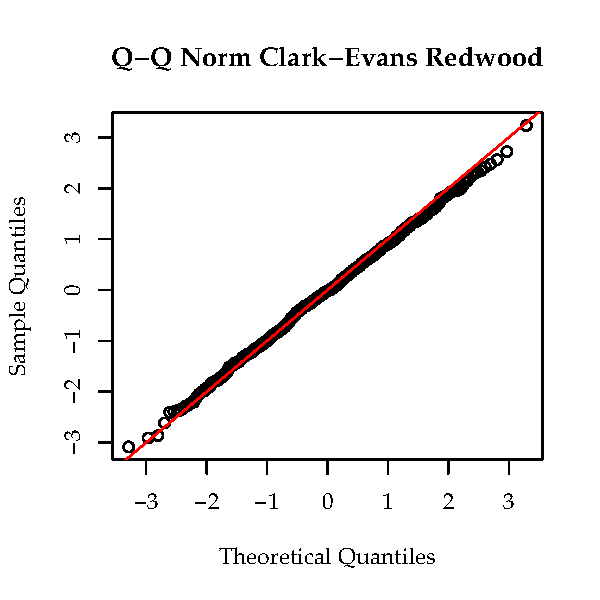
\includegraphics[width=\maxwidth]{figure/prob2g_redwood-1} 

}



\end{knitrout}

\begin{kframe}
\begin{alltt}
\hlcom{# need to calculate the observed statistic}
\hlstd{obs_red} \hlkwb{<-} \hlkwd{nndist}\hlstd{(red)}
\hlstd{obs_mean} \hlkwb{<-} \hlkwd{mean}\hlstd{(obs_red)}
\hlstd{obs_sd} \hlkwb{<-} \hlkwd{sqrt}\hlstd{(}\hlkwd{var}\hlstd{(obs_red))}

\hlstd{all_red} \hlkwb{<-} \hlkwd{data.frame}\hlstd{(}\hlkwd{cbind}\hlstd{(}\hlkwd{c}\hlstd{(obs_mean,obs_sd),}\hlkwd{c}\hlstd{(}\hlkwd{mean}\hlstd{(mean_red),} \hlkwd{sqrt}\hlstd{(}\hlkwd{var}\hlstd{(mean_red))),}
                              \hlkwd{c}\hlstd{(e_hbar.red,}\hlkwd{sqrt}\hlstd{(var_hbar.red))))}
\hlkwd{rownames}\hlstd{(all_red)} \hlkwb{<-} \hlkwd{rownames}\hlstd{(all_cells)}
\hlkwd{colnames}\hlstd{(all_red)} \hlkwb{<-} \hlkwd{c}\hlstd{(}\hlstr{"Observed"}\hlstd{,} \hlstr{"Simulated"}\hlstd{,} \hlstr{"Corrected"}\hlstd{)}

\hlkwd{print}\hlstd{(}\hlkwd{xtable}\hlstd{(all_red,} \hlkwc{align} \hlstd{=} \hlstr{"||l|l|l|l||"}\hlstd{,} \hlkwc{digits} \hlstd{=} \hlkwd{c}\hlstd{(}\hlnum{5}\hlstd{,}\hlnum{5}\hlstd{,}\hlnum{5}\hlstd{,}\hlnum{5}\hlstd{),} \hlkwc{caption} \hlstd{=} \hlstr{"Redwood"}\hlstd{))}
\end{alltt}
\end{kframe}% latex table generated in R 3.3.2 by xtable 1.8-2 package
% Fri Feb  3 11:41:28 2017
\begin{table}[ht]
\centering
\begin{tabular}{||l|l|l|l||}
  \hline
 & Observed & Simulated & Corrected \\ 
  \hline
Mean(Hbar) & 0.03928 & 0.06702 & 0.06713 \\ 
  SD(Hbar) & 0.02590 & 0.00455 & 0.00481 \\ 
   \hline
\end{tabular}
\caption{Redwood} 
\end{table}


\begin{knitrout}\footnotesize
\definecolor{shadecolor}{rgb}{0.969, 0.969, 0.969}\color{fgcolor}\begin{kframe}
\begin{alltt}
\hlstd{lb.red} \hlkwb{<-} \hlstd{e_hbar.red} \hlopt{-} \hlnum{1.96}\hlopt{*}\hlkwd{sqrt}\hlstd{(var_hbar.red)}
\hlstd{ub.red} \hlkwb{<-} \hlstd{e_hbar.red} \hlopt{+} \hlnum{1.96}\hlopt{*}\hlkwd{sqrt}\hlstd{(var_hbar.red)}
\end{alltt}
\end{kframe}
\end{knitrout}

I am 95\% confident the true mean distance for the redwood data is between 0.0577 and 0.0766. The observed mean distance for the cells data was 0.0393 yielding strong evidence of regularity in the redwood data at the 95\% confidence level.

\end{enumerate}

\item %3
{\it I am sending you a copy of a paper by Peter Diggle on the use of K and cross K functions in the analysis of spatial point patterns. The data he is referring to are in the amacrine data set in the spatstat library in R. Read the paper and reproduce the analysis. The data are in spatstat (use the command data(amacrine). You do not have to carry out the significance tests he refers to but I would like for you to take the same approach I took on the analysis of the betacells data set we discussed in class. Write up a summary of your analysis. Pay attention to the distinction between the independence and random labelling hypotheses.}

\begin{knitrout}\footnotesize
\definecolor{shadecolor}{rgb}{0.969, 0.969, 0.969}\color{fgcolor}\begin{kframe}
\begin{alltt}
\hlkwd{data}\hlstd{(}\hlstr{"amacrine"}\hlstd{)}
\hlkwd{plot}\hlstd{(amacrine,} \hlkwc{quiet} \hlstd{=} \hlnum{TRUE}\hlstd{)}
\end{alltt}
\end{kframe}

{\centering 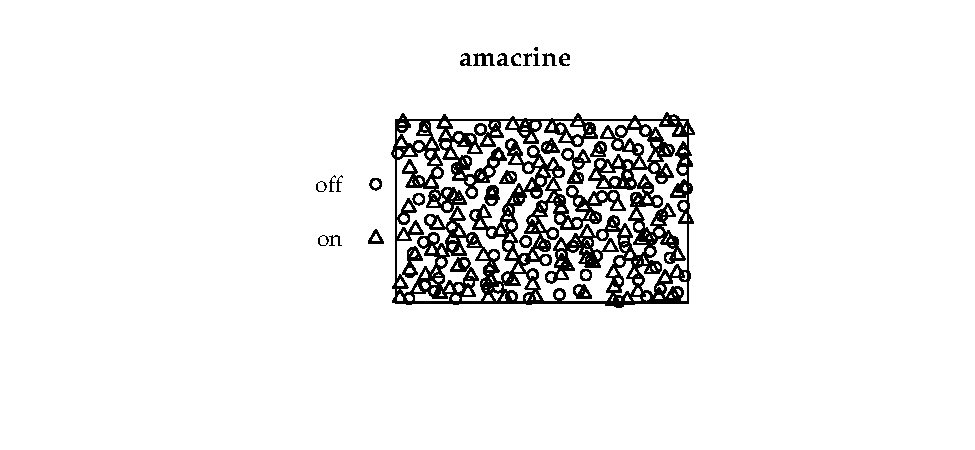
\includegraphics[width=\maxwidth]{figure/prob3-1} 

}


\begin{kframe}\begin{alltt}
\hlcom{#use K it suggests regularity}
\hlkwd{plot}\hlstd{(}\hlkwd{envelope}\hlstd{(amacrine,} \hlkwc{fun} \hlstd{=} \hlstr{"Kest"}\hlstd{,} \hlkwc{correction} \hlstd{=} \hlstr{"iso"}\hlstd{,} \hlkwc{verbose} \hlstd{=} \hlnum{FALSE}\hlstd{),} \hlkwc{main} \hlstd{=} \hlstr{"Kest Iso Correction"}\hlstd{)}
\end{alltt}
\end{kframe}

{\centering 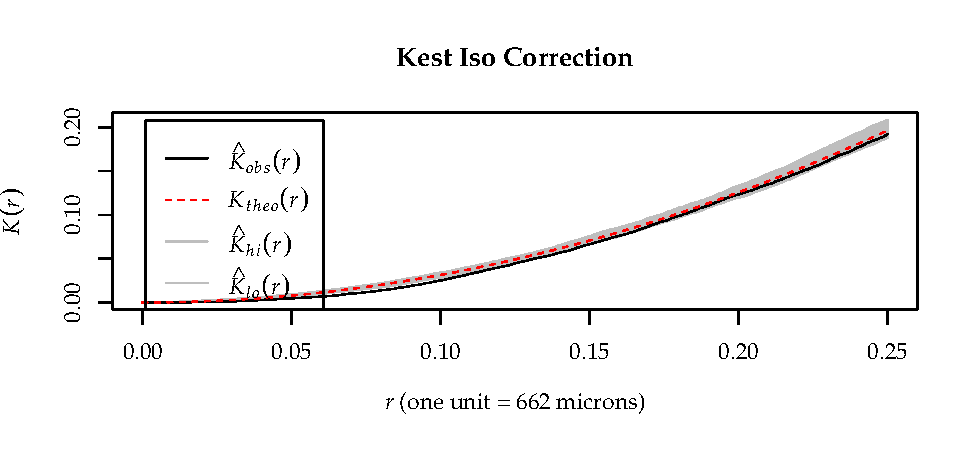
\includegraphics[width=\maxwidth]{figure/prob3-2} 

}


\begin{kframe}\begin{alltt}
\hlkwd{plot}\hlstd{(}\hlkwd{envelope}\hlstd{(amacrine,} \hlkwc{fun} \hlstd{=} \hlstr{"Lest"}\hlstd{,} \hlkwc{correction} \hlstd{=} \hlstr{"iso"}\hlstd{,} \hlkwc{verbose} \hlstd{=} \hlnum{FALSE}\hlstd{),} \hlkwc{main} \hlstd{=} \hlstr{"Lest Iso Correction"}\hlstd{)}
\end{alltt}
\end{kframe}

{\centering 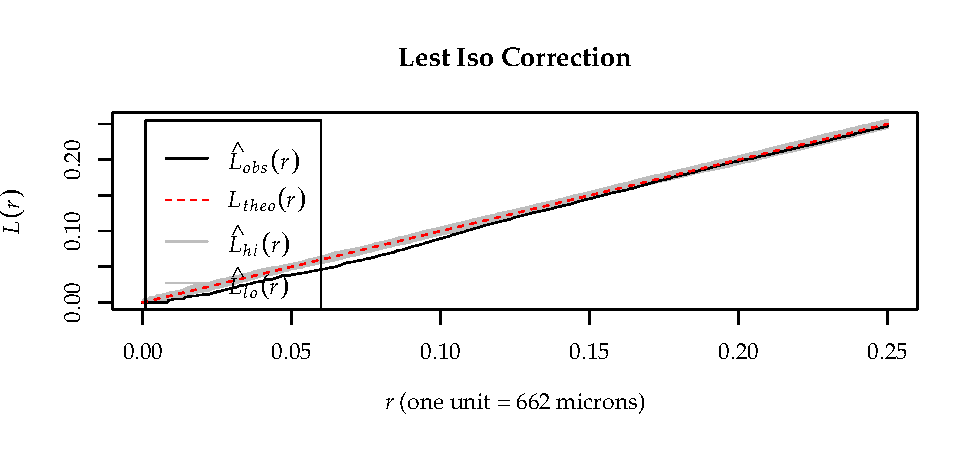
\includegraphics[width=\maxwidth]{figure/prob3-3} 

}


\begin{kframe}\begin{alltt}
\hlkwd{plot}\hlstd{(}\hlkwd{envelope}\hlstd{(amacrine,} \hlkwc{fun} \hlstd{=} \hlstr{"Lest"}\hlstd{,} \hlkwc{global} \hlstd{=} \hlnum{TRUE}\hlstd{,} \hlkwc{correction} \hlstd{=} \hlstr{"iso"}\hlstd{,} \hlkwc{verbose} \hlstd{=} \hlnum{FALSE}\hlstd{),} \hlkwc{main} \hlstd{=} \hlstr{"Lest Iso Correction Global"}\hlstd{)}
\end{alltt}
\end{kframe}

{\centering 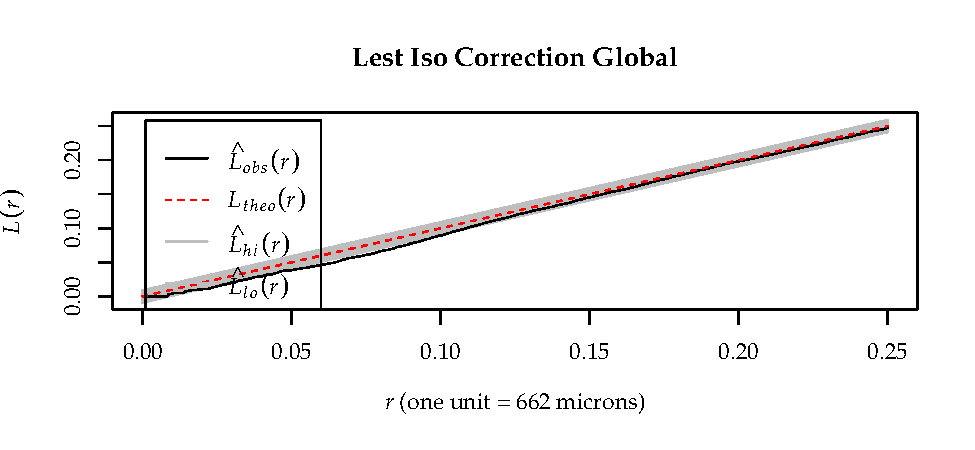
\includegraphics[width=\maxwidth]{figure/prob3-4} 

}


\begin{kframe}\begin{alltt}
\hlstd{off} \hlkwb{<-} \hlkwd{split}\hlstd{(amacrine)}\hlopt{$}\hlstd{off}
\hlstd{on} \hlkwb{<-} \hlkwd{split}\hlstd{(amacrine)}\hlopt{$}\hlstd{on}

\hlkwd{plot}\hlstd{(}\hlkwd{envelope}\hlstd{(off,} \hlkwc{fun} \hlstd{=} \hlstr{"Lest"}\hlstd{,} \hlkwc{correction} \hlstd{=} \hlstr{"iso"}\hlstd{,} \hlkwc{verbose} \hlstd{=} \hlnum{FALSE}\hlstd{), .}\hlopt{-}\hlstd{r}\hlopt{~}\hlstd{r,} \hlkwc{ylab} \hlstd{=} \hlstr{"L(r) - r"}\hlstd{,} \hlkwc{main} \hlstd{=} \hlstr{"Lest Iso Correction Off"}\hlstd{)}
\end{alltt}
\end{kframe}

{\centering 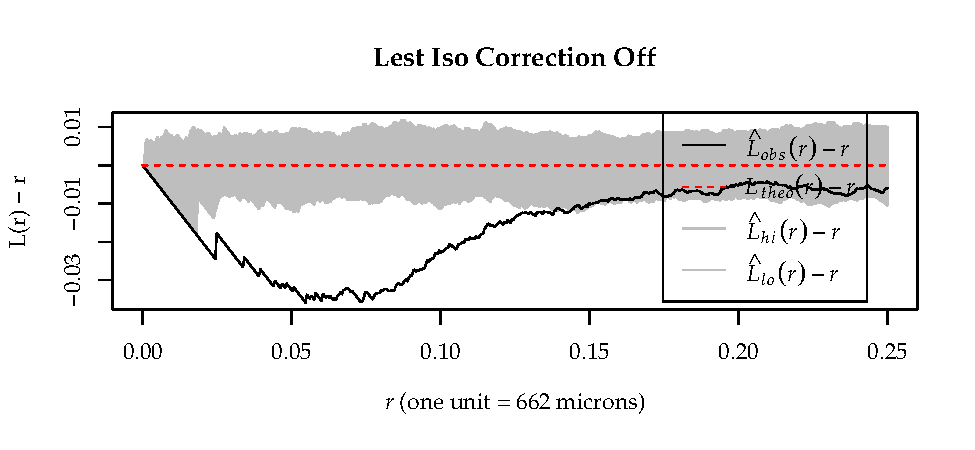
\includegraphics[width=\maxwidth]{figure/prob3-5} 

}


\begin{kframe}\begin{alltt}
\hlkwd{plot}\hlstd{(}\hlkwd{envelope}\hlstd{(on,} \hlkwc{fun} \hlstd{=} \hlstr{"Lest"}\hlstd{,} \hlkwc{correction} \hlstd{=} \hlstr{"iso"}\hlstd{,} \hlkwc{verbose} \hlstd{=} \hlnum{FALSE}\hlstd{), .}\hlopt{-}\hlstd{r}\hlopt{~}\hlstd{r,} \hlkwc{ylab} \hlstd{=} \hlstr{"L(r) - r"}\hlstd{,} \hlkwc{main} \hlstd{=} \hlstr{"Lest Iso Correction On"}\hlstd{)}
\end{alltt}
\end{kframe}

{\centering 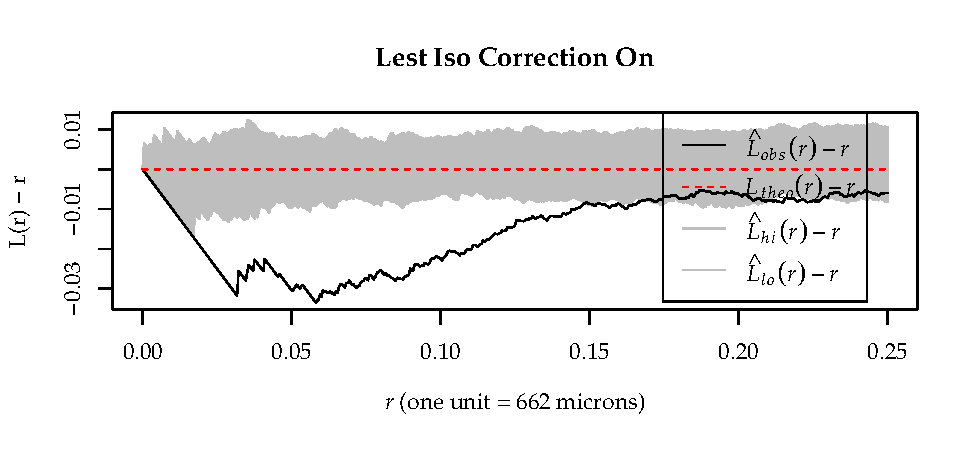
\includegraphics[width=\maxwidth]{figure/prob3-6} 

}


\begin{kframe}\begin{alltt}
\hlkwd{plot}\hlstd{(}\hlkwd{envelope}\hlstd{(amacrine,} \hlkwc{fun} \hlstd{=} \hlstr{"Lcross"}\hlstd{,} \hlkwc{correction} \hlstd{=} \hlstr{"iso"}\hlstd{,} \hlkwc{verbose} \hlstd{=} \hlnum{FALSE}\hlstd{), .}\hlopt{-}\hlstd{r}\hlopt{~}\hlstd{r,} \hlkwc{ylab} \hlstd{=} \hlstr{"L(r) - r"}\hlstd{,} \hlkwc{main} \hlstd{=} \hlstr{"Lcross Iso Correction"}\hlstd{)}
\end{alltt}
\end{kframe}

{\centering 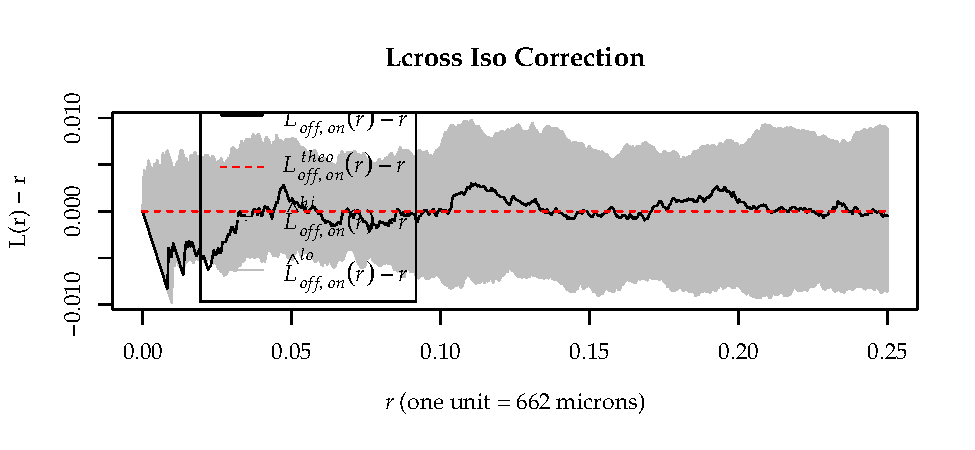
\includegraphics[width=\maxwidth]{figure/prob3-7} 

}


\begin{kframe}\begin{alltt}
\hlkwd{require}\hlstd{(splancs)}
\hlstd{amacrine.poly} \hlkwb{<-} \hlkwd{list}\hlstd{(}\hlkwc{x}\hlstd{=}\hlkwd{c}\hlstd{(off}\hlopt{$}\hlstd{x, on}\hlopt{$}\hlstd{x),} \hlkwc{y}\hlstd{=}\hlkwd{c}\hlstd{(off}\hlopt{$}\hlstd{y, on}\hlopt{$}\hlstd{y))}

\hlcom{# from the paper, make max dist = 0.25*min(side(rectangle(A)))}
\hlcom{# shorter side = height = 1}
\hlcom{# 0.25*1 = 0.25}
\end{alltt}
\end{kframe}
\end{knitrout}

Let 11 = on and 22 = off.


$H_{0}$: $K_{11} = K_{22}$; random labelling

$H_{A}$: $K_{11} \neq K_{22}$; no random labelling

There is no evidence against random labelling as the difference in estimated K functions between the on and off cells lies within the simulation envelopes. 


\begin{knitrout}\footnotesize
\definecolor{shadecolor}{rgb}{0.969, 0.969, 0.969}\color{fgcolor}\begin{kframe}
\begin{alltt}
\hlcom{# random labelling}
\hlcom{# ho: randomly labelling}
\hlcom{# no evidence against random labelling}
\hlstd{h} \hlkwb{<-} \hlkwd{c}\hlstd{(}\hlkwd{seq}\hlstd{(}\hlnum{0}\hlstd{,}\hlnum{0.25}\hlstd{,}\hlkwc{by}\hlstd{=}\hlnum{0.01}\hlstd{))}
\hlstd{khat.on} \hlkwb{<-} \hlkwd{khat}\hlstd{(}\hlkwd{as.points}\hlstd{(on),} \hlkwd{bboxx}\hlstd{(}\hlkwd{bbox}\hlstd{(}\hlkwd{as.points}\hlstd{(amacrine.poly))),} \hlkwc{s} \hlstd{= h)}
\hlstd{khat.off} \hlkwb{<-} \hlkwd{khat}\hlstd{(}\hlkwd{as.points}\hlstd{(off),} \hlkwd{bboxx}\hlstd{(}\hlkwd{bbox}\hlstd{(}\hlkwd{as.points}\hlstd{(amacrine.poly))),} \hlkwc{s} \hlstd{= h)}

\hlstd{kdiff} \hlkwb{<-} \hlstd{khat.on}\hlopt{-}\hlstd{khat.off}
\hlkwd{plot}\hlstd{(h, kdiff,} \hlkwc{xlab}\hlstd{=}\hlstr{"Distance"}\hlstd{,} \hlkwc{ylab}\hlstd{=}\hlkwd{expression}\hlstd{(}\hlkwd{hat}\hlstd{(K)[}\hlnum{11}\hlstd{]} \hlopt{-} \hlkwd{hat}\hlstd{(k)[}\hlnum{22}\hlstd{]),}
     \hlkwc{type}\hlstd{=}\hlstr{"l"}\hlstd{,} \hlkwc{main}\hlstd{=}\hlstr{"simulation envelopes, random labelling"}\hlstd{,} \hlkwc{ylim}\hlstd{=}\hlkwd{c}\hlstd{(}\hlopt{-}\hlnum{.05}\hlstd{,}\hlnum{.05}\hlstd{))}

\hlstd{env.lab} \hlkwb{<-} \hlkwd{Kenv.label}\hlstd{(}\hlkwd{as.points}\hlstd{(on),}\hlkwd{as.points}\hlstd{(off),}
                      \hlkwd{bboxx}\hlstd{(}\hlkwd{bbox}\hlstd{(}\hlkwd{as.points}\hlstd{(amacrine.poly))),} \hlkwc{nsim} \hlstd{=} \hlnum{99}\hlstd{,}\hlkwc{s}\hlstd{=h,} \hlkwc{quiet} \hlstd{=} \hlnum{TRUE}\hlstd{)}

\hlkwd{lines}\hlstd{(h, env.lab}\hlopt{$}\hlstd{upper,} \hlkwc{lty}\hlstd{=}\hlnum{2}\hlstd{)}
\hlkwd{lines}\hlstd{(h, env.lab}\hlopt{$}\hlstd{lower,} \hlkwc{lty}\hlstd{=}\hlnum{2}\hlstd{)}
\end{alltt}
\end{kframe}

{\centering 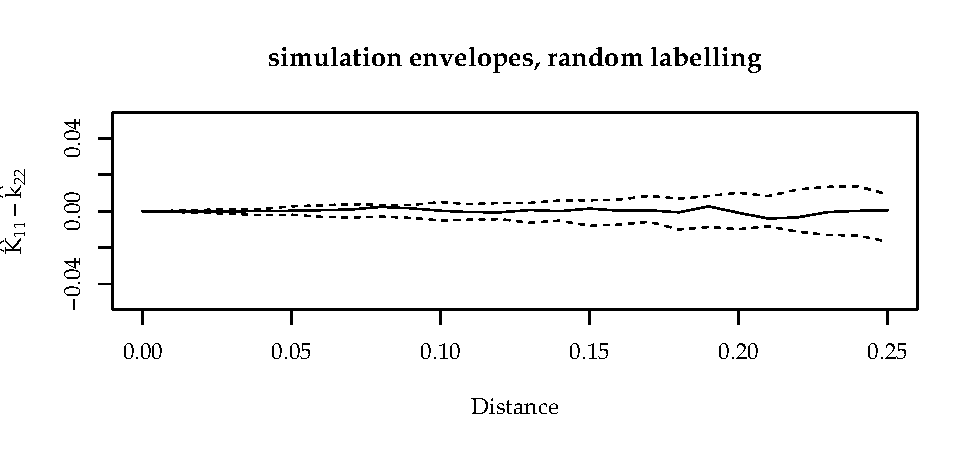
\includegraphics[width=\maxwidth]{figure/rand_lab-1} 

}



\end{knitrout}

$H_{0}$: $K_{11} = K_{12}$; random labelling

$H_{A}$: $K_{11} \neq K_{12}$; no random labelling

There is evidence against random labelling as the difference line lies outside the simulation envelopes. 

\begin{knitrout}\footnotesize
\definecolor{shadecolor}{rgb}{0.969, 0.969, 0.969}\color{fgcolor}\begin{kframe}
\begin{alltt}
\hlcom{## D function calculation - cross K and K.on}
\hlcom{# First calculate the observed value of D}
\hlcom{# I had to modify the code a bit because betacells}
\hlcom{# has two types of marks and Kcross had trouble with that.}
\hlcom{# I only needed to work with}
\hlcom{# the binary type (on,off) marks.}
\hlstd{amacrine.new}\hlkwb{<-}\hlstd{amacrine}
\hlstd{amacrine.new}\hlopt{$}\hlstd{marks}\hlkwb{<-}\hlstd{amacrine}\hlopt{$}\hlstd{marks}
\hlstd{amacrine.newoff}\hlkwb{<-}\hlkwd{split}\hlstd{(amacrine,}\hlkwc{f}\hlstd{=}\hlkwd{marks}\hlstd{(amacrine.new))}\hlopt{$}\hlstd{off}
\hlstd{amacrine.newon}\hlkwb{<-}\hlkwd{split}\hlstd{(amacrine,}\hlkwc{f}\hlstd{=}\hlkwd{marks}\hlstd{(amacrine.new))}\hlopt{$}\hlstd{on}
\hlcom{## Set up}
\hlstd{mark.vec}\hlkwb{<-}\hlkwd{marks}\hlstd{(amacrine.new)}
\hlstd{sim.mat}\hlkwb{<-}\hlkwd{matrix}\hlstd{(}\hlnum{0}\hlstd{,}\hlkwc{nrow}\hlstd{=}\hlnum{513}\hlstd{,}\hlkwc{ncol}\hlstd{=}\hlnum{100}\hlstd{)}
\hlstd{Dfun}\hlkwb{<-}\hlkwd{Kcross}\hlstd{(amacrine.new)}\hlopt{$}\hlstd{iso} \hlopt{-} \hlkwd{Kest}\hlstd{(amacrine.newon)}\hlopt{$}\hlstd{iso}
\hlstd{sim.mat[,}\hlnum{1}\hlstd{]}\hlkwb{<-}\hlstd{Dfun}
\hlcom{## Loop}
\hlkwa{for}\hlstd{(i} \hlkwa{in} \hlnum{2}\hlopt{:}\hlnum{100}\hlstd{)\{}
   \hlstd{indx}\hlkwb{<-}\hlkwd{sample}\hlstd{(}\hlnum{1}\hlopt{:}\hlnum{294}\hlstd{,}\hlkwc{rep}\hlstd{=F)}
   \hlstd{amacrine.new}\hlopt{$}\hlstd{marks}\hlkwb{<-}\hlstd{amacrine.new}\hlopt{$}\hlstd{marks[indx]}
   \hlstd{sim.mat[,i]}\hlkwb{<-}\hlkwd{Kcross}\hlstd{(amacrine.new)}\hlopt{$}\hlstd{iso} \hlopt{-}
               \hlkwd{Kest}\hlstd{(amacrine.newon)}\hlopt{$}\hlstd{iso}
\hlstd{\}}
\hlstd{Dfun.min}\hlkwb{<-}\hlkwd{apply}\hlstd{(sim.mat[,}\hlopt{-}\hlnum{1}\hlstd{],}\hlnum{1}\hlstd{,min)}
\hlstd{Dfun.max}\hlkwb{<-}\hlkwd{apply}\hlstd{(sim.mat[,}\hlopt{-}\hlnum{1}\hlstd{],}\hlnum{1}\hlstd{,max)}
\hlstd{hdist}\hlkwb{<-}\hlkwd{Kest}\hlstd{(amacrine)}\hlopt{$}\hlstd{r}
\hlstd{minD} \hlkwb{<-} \hlkwd{min}\hlstd{(Dfun.min)}
\hlstd{maxD} \hlkwb{<-} \hlkwd{max}\hlstd{(Dfun.max)}
\hlstd{maxHdist} \hlkwb{<-} \hlkwd{max}\hlstd{(hdist)}
\hlkwd{plot}\hlstd{(}\hlkwd{c}\hlstd{(}\hlnum{0}\hlstd{,maxHdist),}\hlkwd{c}\hlstd{(minD,maxD),}\hlkwc{type}\hlstd{=}\hlstr{"n"}\hlstd{,}\hlkwc{xlab}\hlstd{=}\hlstr{"distance"}\hlstd{,}\hlkwc{ylab}\hlstd{=}\hlstr{"D function"}\hlstd{)}
\hlkwd{abline}\hlstd{(}\hlkwc{h}\hlstd{=}\hlnum{0}\hlstd{)}
\hlkwd{lines}\hlstd{(hdist,Dfun.min,}\hlkwc{lty}\hlstd{=}\hlnum{2}\hlstd{)}
\hlkwd{lines}\hlstd{(hdist,Dfun.max,}\hlkwc{lty}\hlstd{=}\hlnum{2}\hlstd{)}
\hlkwd{lines}\hlstd{(hdist,Dfun)}
\end{alltt}
\end{kframe}

{\centering 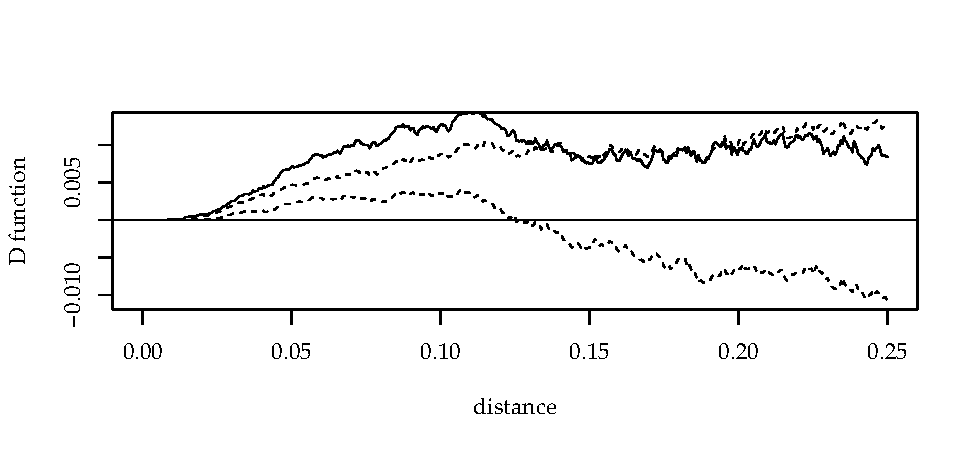
\includegraphics[width=\maxwidth]{figure/rand_label12-1} 

}



\end{knitrout}

$H_{0}:$ independence

$H_{A}$: no independence

There is no evidence against independence as the line lies within the envelope.

\begin{knitrout}\footnotesize
\definecolor{shadecolor}{rgb}{0.969, 0.969, 0.969}\color{fgcolor}\begin{kframe}
\begin{alltt}
\hlstd{amacrine.poly} \hlkwb{<-} \hlkwd{list}\hlstd{(}\hlkwc{x}\hlstd{=}\hlkwd{c}\hlstd{(amacrine.newon}\hlopt{$}\hlstd{x, amacrine.newoff}\hlopt{$}\hlstd{x),}
\hlkwc{y}\hlstd{=}\hlkwd{c}\hlstd{(amacrine.newon}\hlopt{$}\hlstd{y,amacrine.newoff}\hlopt{$}\hlstd{y))}
\hlcom{# specify the range of radii for the plot}
\hlstd{h}\hlkwb{<-}\hlkwd{seq}\hlstd{(}\hlnum{0}\hlstd{,}\hlnum{0.25}\hlstd{,}\hlnum{.005}\hlstd{)}
\hlcom{# Produce a modified cross L function}
\hlstd{Lcross.plot}\hlkwb{<-}\hlkwd{sqrt}\hlstd{(}\hlkwd{k12hat}\hlstd{(}\hlkwd{as.points}\hlstd{(amacrine.newon),}\hlkwd{as.points}\hlstd{(amacrine.newoff),}
             \hlkwd{bboxx}\hlstd{(}\hlkwd{bbox}\hlstd{(}\hlkwd{as.points}\hlstd{(amacrine.poly))),h)}\hlopt{/}\hlstd{pi)} \hlopt{-} \hlstd{h}
\hlkwd{plot}\hlstd{(h,Lcross.plot,} \hlkwc{xlab}\hlstd{=}\hlstr{"distance"}\hlstd{,}
     \hlkwc{ylab}\hlstd{=}\hlkwd{expression}\hlstd{(}\hlkwd{hat}\hlstd{(L)[}\hlnum{12}\hlstd{]),} \hlkwc{ylim} \hlstd{=} \hlkwd{c}\hlstd{(}\hlopt{-}\hlnum{0.01}\hlstd{,}\hlnum{0.01}\hlstd{),}\hlkwc{type}\hlstd{=}\hlstr{"l"}\hlstd{,}
     \hlkwc{main}\hlstd{=}\hlstr{"Simulation envelopes, random toroidal shifts"}\hlstd{)}
\hlcom{# Get the bounds on the simulation envelope.}
\hlstd{Lcross.env}\hlkwb{<-} \hlkwd{Kenv.tor}\hlstd{(}\hlkwd{as.points}\hlstd{(amacrine.newon),} \hlkwd{as.points}\hlstd{(amacrine.newoff),}
     \hlkwd{bboxx}\hlstd{(}\hlkwd{bbox}\hlstd{(}\hlkwd{as.points}\hlstd{(amacrine.poly))),} \hlkwc{nsim}\hlstd{=}\hlnum{499}\hlstd{,} \hlkwc{s}\hlstd{=h,} \hlkwc{quiet} \hlstd{=} \hlnum{TRUE}\hlstd{)}
\hlkwd{lines}\hlstd{(h,} \hlkwd{sqrt}\hlstd{(Lcross.env}\hlopt{$}\hlstd{upper}\hlopt{/}\hlstd{pi)}\hlopt{-}\hlstd{h,} \hlkwc{lty}\hlstd{=}\hlnum{2}\hlstd{)}
\hlkwd{lines}\hlstd{(h,} \hlkwd{sqrt}\hlstd{(Lcross.env}\hlopt{$}\hlstd{lower}\hlopt{/}\hlstd{pi)}\hlopt{-}\hlstd{h,} \hlkwc{lty}\hlstd{=}\hlnum{2}\hlstd{)}
\end{alltt}
\end{kframe}

{\centering 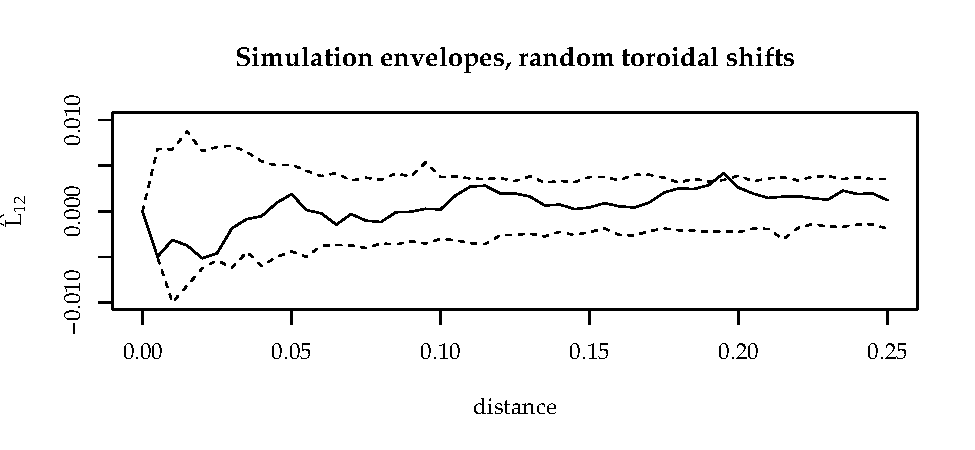
\includegraphics[width=\maxwidth]{figure/ind-1} 

}



\end{knitrout}

Overall, CSR is violated as we cannot assume random labelling.

\end{enumerate}

\end{document}

